\documentclass[journal]{IEEEtran}

\usepackage{amsmath,amssymb}
\usepackage{graphicx}
\usepackage{booktabs}
\usepackage{multirow}
\usepackage{xcolor}
\usepackage[hidelinks,hypertexnames=false]{hyperref}
\usepackage{algorithm}
\usepackage{algorithmic}
\usepackage{balance}

\graphicspath{{../figures/}{../../Experiment/core_code/outputs/visualizations/}}

\newcommand{\ours}{CARE}  % Collapse-Aware REpair
\newcommand{\ie}{\textit{i.e.}}
\newcommand{\eg}{\textit{e.g.}}
\newcommand{\etal}{\textit{et al.}\@}

\begin{document}

\title{Class Collapse in Encrypted Traffic Classifiers: Discovery and Label-Efficient Repair}

\author{
  Junwei Xiao
  \thanks{J.~Xiao is with the School of Advanced Technology, Xi'an Jiaotong-Liverpool University, Suzhou, China. E-mail: Junwei.Xiao@xjtlu.edu.cn}
}

\maketitle

% ============================================================
\begin{abstract}
Deep-learning encrypted traffic classifiers degrade after deployment due to concept drift.
We identify a previously unstudied failure mode---the \textit{absorber-collapse pattern}---in which a few dominant classes systematically absorb predictions from victim classes, driving them to near-zero recall.
On CESNET-TLS-Year22, 12 of 178 classes collapse below 0.1 recall within nine months; five representative test-time adaptation methods all leave collapse-class F1 below 0.03.
We propose \ours{} (\textbf{C}ollapse-\textbf{A}ware \textbf{RE}pair), a label-efficient maintenance framework that monitors per-class collapse risk, selects 1{,}000 informative target samples via pair-agnostic margin or BADGE sampling, and repairs the classification head through few-label fine-tuning, all-class source replay, and knowledge distillation.
An unsupervised detection module serves as a diagnostic monitor, flagging at-risk classes without labels.
Under strict evaluation (queried samples excluded, five seeds), \ours{}-BADGE raises macro-F1 from 0.629 to $0.700{\pm}0.003$ and collapse-class F1 from 0.028 to $0.333{\pm}0.040$; the lightweight \ours{}-Margin variant reaches $0.686{\pm}0.001$ in under one second.
The framework is consistent across drift severity, architectures, and training seeds.
\end{abstract}

\begin{IEEEkeywords}
Encrypted traffic classification, concept drift, class collapse, label-efficient maintenance, active learning
\end{IEEEkeywords}

% ============================================================
\section{Introduction}
\label{sec:intro}

% P1: Problem - drift in traffic classifiers
Deep learning has become the dominant approach for encrypted traffic classification, achieving impressive accuracy on benchmark datasets~\cite{lin2022etbert, zhao2023yatc, pacheco2019towards, wang2019survey}.
However, a growing body of evidence shows that these classifiers degrade rapidly after deployment.
Soukup~\etal{}~\cite{soukup2025drift} identify 28 frequently drifting classes on CESNET-TLS-Year22, while Malekghaini~\etal{}~\cite{malekghaini2023drift} observe F1 declining from 0.95 to 0.60 over several months on ISP-scale data.
The causes are diverse: application version updates alter protocol behavior, TLS certificate rotations change handshake fingerprints, and CDN migrations shift IP ranges and packet-size distributions~\cite{soukup2025drift, lu2019learning, gama2014survey}.

% P2: Existing solutions and their limitations
Existing approaches to this problem span three categories.
Periodic retraining with freshly labeled data~\cite{chen2025selfevolving} is effective but costly.
Unsupervised test-time adaptation (TTA) from computer vision~\cite{wang2021tent, niu2022eata, niu2023sar} avoids labeling but, as we demonstrate, is ineffective for traffic classifiers.
Standard active learning~\cite{settles2009active, sener2018coreset, ash2020badge} can select informative samples, but generic strategies are not designed for the specific failure mode we identify.
This motivates a different approach: \textit{targeted, label-efficient maintenance} that diagnoses which classes have collapsed and repairs them with minimal annotation cost.

% P3: Our finding - absorber-collapse pattern
We identify a previously unstudied failure mode that we term the \textit{absorber-collapse pattern}.
Through systematic confusion analysis on the CESNET-TLS-Year22 dataset~\cite{hynek2024cesnet}, we discover that performance degradation is not uniform across classes.
Instead, a small number of dominant ``absorber'' classes systematically attract predictions away from ``victim'' classes, causing the victims to collapse to near-zero recall.
For example, class~56 is misclassified as class~96 (its absorber) at a rate of 25.2\%, while class~163 loses 41.8\% of its predictions to class~46.
This pattern affects 12 out of 178 classes within nine months, rendering them effectively undetectable.
Critically, we show that five representative TTA methods---including SAR~\cite{niu2023sar} and NOTE~\cite{gong2022note} under traffic-adapted implementations---produce collapse-class F1 scores below 0.03, offering no improvement over a static baseline.

% P4: Our solution - CARE
We propose \ours{}, a collapse-aware repair framework with three complementary components:
\begin{enumerate}
  \item \textbf{Few-label fine-tuning.} We actively select $B{=}1{,}000$ informative target samples via margin or BADGE sampling and fine-tune only the classification head, keeping the encoder frozen.
  \item \textbf{All-class source replay.} $k{=}5$ exemplars per class (890 samples total) from labeled reference-period data are mixed into fine-tuning to prevent catastrophic forgetting. We use M4 as the reference period; an equivalence experiment confirms that using the training month (M3) yields nearly identical results (macro-F1: $0.672{\pm}0.002$ vs.\ $0.673{\pm}0.001$), so the replay data can be sourced from either the training pipeline or a nearby labeled period.
  \item \textbf{Knowledge distillation.} A KL-divergence loss between the updated and original heads on replay samples anchors the overall prediction behavior.
\end{enumerate}
An unsupervised detection module, based on five complementary signals (prediction count ratio, Fr\'{e}chet distance, margin drop, confidence drop, entropy rise), monitors per-class health and signals when repair may be needed---it serves as a diagnostic monitor, not as a mechanism for selecting replay classes or guiding sample selection.

% P5: Results highlight
We first establish that unsupervised TTA methods, under our traffic-adapted implementations, do not address class collapse (all produce collapse-class F1 ${<}0.03$), and that uncertainty-based active learning strategies (entropy, coreset) with the same label budget perform \textit{worse} than no adaptation.
Under strict evaluation (queried samples excluded, five seeds), \ours{}-BADGE raises macro-F1 from 0.629 to $0.700{\pm}0.003$ and collapse-class F1 from 0.028 to $0.333{\pm}0.040$ ($12{\times}$) using 1{,}000 target labels ($<$0.3\% of the test set) plus 890 all-class replay samples; a lightweight margin variant achieves $0.686{\pm}0.001$ with sub-second selection time.
A clean component ablation confirms that each ingredient---fine-tuning, replay, and distillation---contributes independently, with the full combination yielding the best trade-off between collapse repair and stable-class preservation.
\ours{} is consistent across architectures (CNN and Transformer) and drift severity (M7--M12). Prototype replay enables exemplar-free deployment.

Our contributions are:
\begin{enumerate}
  \item \textbf{Failure mode discovery.} We identify and formalize the \textit{absorber-collapse pattern}---a systematic failure mode where dominant classes absorb victim-class predictions under concept drift, distinct from uniform degradation or class imbalance. Via Fisher discriminant analysis, we characterize two mechanisms---feature drift (9 of 12 classes) and boundary shift (3 of 12)---with per-class quantitative evidence and recovery analysis for all 12 collapse classes (\S\ref{sec:analysis}).
  \item \textbf{Negative results.} We show that five TTA methods (collapse F1 ${<}0.03$) and two standard active learning strategies (entropy, coreset) all fail on class collapse, establishing it as a distinct problem that existing approaches do not address (\S\ref{sec:tta_eval}, \S\ref{sec:al_baselines}).
  \item \textbf{Collapse-aware evaluation.} We introduce complementary metrics---collapse-class F1, per-class recovery status, stable-class preservation, and strict query exclusion---that reveal failure modes invisible to aggregate macro-F1 (\S\ref{sec:experiments}).
  \item \textbf{Label-efficient maintenance framework.} We propose \ours{}, a validated maintenance protocol combining margin/BADGE selection, all-class replay, head-only fine-tuning, and knowledge distillation. Each component's contribution is isolated via a 7-configuration ablation; an unsupervised detection module (recall $\geq$0.80) serves as a diagnostic monitor (\S\ref{sec:method}, \S\ref{sec:experiments}).
\end{enumerate}


% ============================================================
\section{Related Work}
\label{sec:related}

\subsection{Concept Drift in Encrypted Traffic Classification}

Encrypted traffic classifiers rely on statistical features of packet sequences that are inherently non-stationary under protocol and infrastructure changes~\cite{rezaei2019deep, soukup2025drift, malekghaini2023drift}.
Soukup~\etal{}~\cite{soukup2025drift} identified 28 frequently drifting classes on CESNET-TLS-Year22 but analyzed only per-class F1 trajectories; Malekghaini~\etal{}~\cite{malekghaini2023drift} noted absorber-like behavior (``Web is the class most misclassified flows are confused with'') without further analysis.
Jerabek~\etal{}~\cite{jerabek2025eval} showed that random splitting inflates performance by $\geq$3.5pp vs.\ time-based evaluation.
Chen~\etal{}~\cite{chen2025selfevolving} proposed pseudo-label-based fine-tuning but explicitly excluded per-class analysis.
None of these works identifies the systematic absorber--victim pattern we formalize here.

\subsection{Test-Time Adaptation}

TTA methods update model parameters at inference time without labels: Tent~\cite{wang2021tent}, EATA~\cite{niu2022eata}, SAR~\cite{niu2023sar}, CoTTA~\cite{wang2022cotta}, and NOTE~\cite{gong2022note}.
These were designed for image-corruption benchmarks (ImageNet-C) and assume BatchNorm-based architectures.
Our classifier uses GroupNorm~\cite{wu2018groupnorm}; we verify that TTA fails on both GroupNorm and BatchNorm variants (\S\ref{sec:bn_verify}), confirming a problem-level rather than architecture-level limitation.

\subsection{Continual Learning for Traffic Classification}

Several methods address class-incremental learning for traffic: ILETC~\cite{zhu2023iletc} (generative replay), MEMENTO~\cite{cerasuolo2024memento} (KD + memory replay), CPN~\cite{cai2024cpn} (contrastive prototypes), and PRIME~\cite{prime2025} (plasticity-aware expansion). The broader CL literature~\cite{delange2022continual} offers EWC~\cite{kirkpatrick2017ewc} and LwF~\cite{li2018lwf} for catastrophic forgetting.
These share technical components with our approach but address a different problem: adding \textit{new} classes. Our problem---repairing \textit{existing} classes collapsed by drift---is complementary and, to our knowledge, previously unstudied.

\subsection{Domain Adaptation, Class Imbalance, and Active Learning}

UDA methods (DANN~\cite{ganin2016dann}, CDAN~\cite{long2018cdan}) assume all classes shift uniformly; absorber-collapse is \textit{class-asymmetric}, making global alignment ineffective.
The pattern superficially resembles class imbalance~\cite{kang2020decoupling, menon2021longtail}, but collapse is \textit{caused by drift}, not inherent data imbalance---standard long-tail remedies cannot address it without test-time labels.
CADE~\cite{yang2021cade} detects drift samples via contrastive explanation but targets novel-class detection.
Liu~\etal{}~\cite{micfoal2023} and NetGuard~\cite{netguard2025} address drift-aware active learning broadly; neither identifies the absorber-collapse pattern. Our experiments show that entropy and coreset selection are counterproductive for collapse repair (\S\ref{sec:al_baselines}).


% ============================================================
\section{Empirical Analysis: Class Collapse Under Drift}
\label{sec:analysis}

\subsection{Problem Formulation}
\label{sec:problem}

Let $f_\phi: \mathcal{X} \to \mathbb{R}^d$ denote a frozen feature encoder and $h_\theta: \mathbb{R}^d \to \mathbb{R}^C$ a classification head, jointly trained on a source period $\mathcal{D}^{\text{src}}$ with $C$ application classes.
At a later target period $t$, the data distribution shifts: $P_t(\mathbf{x}, y) \neq P_{\text{src}}(\mathbf{x}, y)$.
We define a class $c$ as \textit{collapsed} at period $t$ if its recall $R_c^{(t)} = \text{TP}_c / ({\text{TP}_c + \text{FN}_c}) < \tau$ for a threshold $\tau$ (we use $\tau{=}0.1$).
A collapsed class $c$ has a \textit{primary absorber} $a(c) = \arg\max_{j \neq c}\, n_{c \to j}$, where $n_{c \to j}$ counts samples with true label $c$ predicted as $j$.
The goal of collapse-aware repair is: given a small label budget $B \ll |\mathcal{D}^{\text{tgt}}|$ and optional source replay data, update $h_\theta$ so that $R_c^{(t)}$ recovers for collapsed classes while preserving performance on stable classes.

\subsection{Experimental Setup}
\label{sec:setup_analysis}

We use the CESNET-TLS-Year22 dataset~\cite{hynek2024cesnet}, which contains 507.7M TLS flows across 12 months of 2022 from a university network.
We use the \texttt{size=S} split provided by the CESNET DataZoo API, yielding approximately 330K test samples per monthly period across 178 application classes.
Each flow is represented by Per-Packet Information (PPI): packet sizes, directions, and inter-packet times for the first 30 packets.

We train a CNN classifier (3-layer 1D convolution with GroupNorm, 8 groups, 256-dim hidden layer, 178 classes) on March 2022 alone (M3) and evaluate on M4--M12, giving a minimum time gap of one month and maximum of nine months.
Training uses a joint classification + self-supervised objective: cross-entropy loss plus three auxiliary SSL tasks (masked packet-feature prediction, packet-order prediction, and flow-statistics reconstruction) with SSL weight 1.0, mask ratio 0.15, and auxiliary loss weights $\alpha{=}0.2$, $\beta{=}0.1$.
The SSL tasks improve encoder generalization but are not used during \ours{} repair (which freezes the encoder and updates only the classification head).
Training runs for 30 epochs with AdamW~\cite{loshchilov2019adamw} (lr$=10^{-3}$, weight decay$=10^{-4}$), batch size 1024, using the DataZoo default validation split.

\subsection{The Absorber-Collapse Pattern}
\label{sec:absorber}

\begin{figure}[t]
\centering
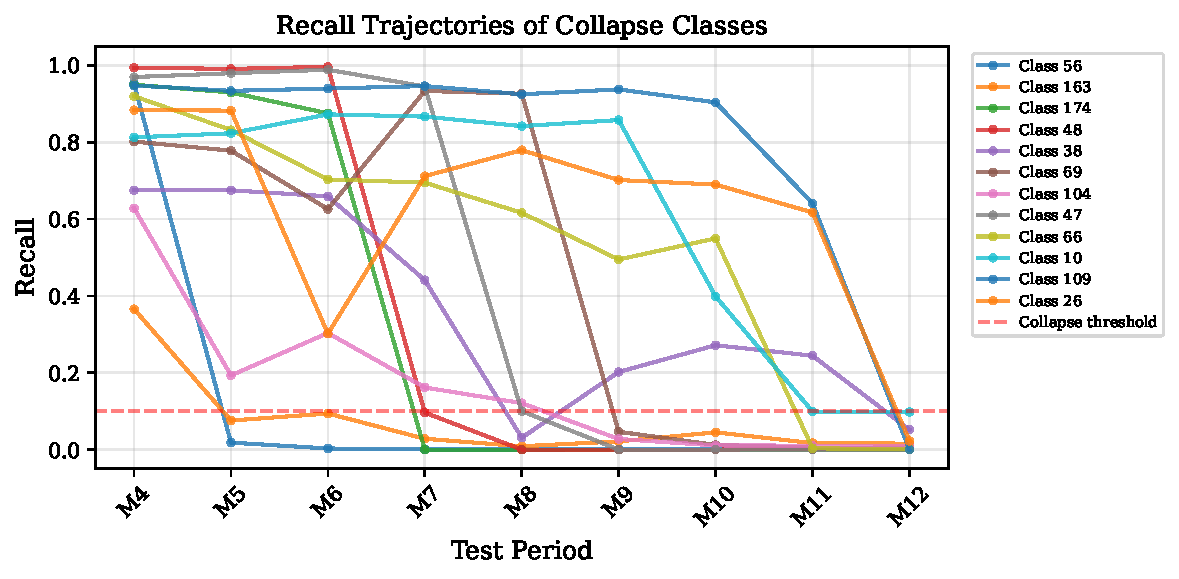
\includegraphics[width=\columnwidth]{fig_collapse_timeline.pdf}
\caption{Recall trajectories of 12 collapse classes on CESNET-TLS-Year22. Classes exhibit both abrupt collapse (\eg{}, class~56 at M5) and gradual decline (\eg{}, class~104 over M5--M9). By M12, all 12 classes fall below the 0.1 recall threshold (dashed line).}
\label{fig:collapse_timeline}
\end{figure}

Figure~\ref{fig:collapse_timeline} shows the recall trajectory of 12 classes that collapse below 0.1 recall by month~12.
The collapses follow two distinct temporal patterns:
\begin{itemize}
  \item \textbf{Abrupt collapse}: Recall drops sharply within one month (\eg{}, class~56 drops from 0.95 to 0.02 at M5 due to certificate rotation).
  \item \textbf{Gradual collapse}: Recall decays steadily over several months (\eg{}, class~104 declines from 0.63 to 0.01 over M3--M9).
\end{itemize}

Crucially, these collapses are not random---each victim class has a \textit{primary absorber}: the dominant confusion target that receives the largest share of the victim's mispredictions.
Table~\ref{tab:absorber_pairs} lists the 12 collapse classes and their top absorbers, with confusion rates ranging from 13.9\% to 46.1\%.

\begin{table}[t]
\centering
\caption{Absorber-collapse pairs at M-2022-12. Each collapsed class has a dominant confusion target (absorber). Confusion rate = fraction of victim samples predicted as the absorber.}
\label{tab:absorber_pairs}
\small
\begin{tabular}{@{}cccccc@{}}
\toprule
Victim & Absorber & Confusion & Victim & Pattern & First \\
Class  & Class    & Rate      & Recall & Type    & Collapse \\
\midrule
56  & 96  & 25.2\% & 0.000 & abrupt  & M5 \\
163 & 46  & 41.8\% & 0.015 & gradual & M5 \\
174 & 2   & 29.2\% & 0.000 & abrupt  & M7 \\
48  & 14  & 39.0\% & 0.001 & abrupt  & M7 \\
38  & 45  & 46.1\% & 0.052 & abrupt  & M8 \\
69  & 105 & 37.7\% & 0.005 & abrupt  & M9 \\
104 & 2   & 21.2\% & 0.010 & gradual & M9 \\
47  & 5   & 45.1\% & 0.000 & gradual & M11 \\
66  & 71  & 13.9\% & 0.001 & abrupt  & M11 \\
10  & 156 & 36.5\% & 0.098 & gradual & M11 \\
109 & 71  & 24.9\% & 0.000 & abrupt  & M12 \\
26  & 13  & 21.6\% & 0.022 & abrupt  & M12 \\
\bottomrule
\end{tabular}
\end{table}

\subsection{Two Mechanisms of Collapse}
\label{sec:mechanisms}

By comparing the Fisher discriminant ratio (inter-class distance / sum of intra-class spreads) between victim--absorber pairs at M4 (pre-collapse) and M12 (post-collapse), we classify each collapse class by the relative change $\Delta J = (J_{\text{M12}} - J_{\text{M4}}) / J_{\text{M4}}$: \textit{feature drift} when $\Delta J < -10\%$ and \textit{boundary shift} when $\Delta J > +20\%$. This yields two distinct mechanisms:

\begin{itemize}
  \item \textbf{Feature drift} (9 of 12 classes, including 56, 174, 104, 109): The victim's feature distribution physically shifts toward the absorber in feature space. The Fisher ratio decreases 14--59\% from M4 to M12 (\eg{}, class~109$\to$71: Fisher drops from 0.875 to 0.361). This occurs when application updates cause the victim's traffic patterns to resemble the absorber's.
  \item \textbf{Boundary shift} (3 of 12 classes: 48, 69, 10): The inter-class distance \emph{increases} (Fisher ratio rises 30--45\%), yet the classifier still absorbs the victim. This suggests the decision boundary shifts due to changes in other classes' distributions, indirectly pushing the victim onto the absorber's side.
\end{itemize}

The two mechanisms have different implications for repair: feature-drift collapse can be addressed by re-anchoring the victim's prototype, while boundary-shift collapse requires recalibrating the decision boundary across multiple classes simultaneously. \ours{}'s combination of targeted fine-tuning and all-class source replay addresses both mechanisms.

\begin{table*}[t]
\centering
\caption{Fisher discriminant ratio analysis for all 12 collapse classes. $J_{\text{M4}}$ and $J_{\text{M12}}$ denote the Fisher ratio (inter-class distance / sum of intra-class spreads) between victim and absorber at M4 and M12, respectively. $\Delta J$ is the relative change. Static and \ours{} recall are at M12.}
\label{tab:fisher}
\scriptsize
\begin{tabular}{@{}r r l rr r rr l@{}}
\toprule
Victim & Abs. & Mechanism & $J_{\text{M4}}$ & $J_{\text{M12}}$ & $\Delta J$(\%) & Static & \ours{} & Status \\
\midrule
\multicolumn{9}{@{}l}{\textit{Feature drift --- victim shifts toward absorber ($\Delta J < -10\%$)}} \\
56  & 96  & feat.\ drift & 0.886 & 0.627 & $-$29 & .000 & .793 & recov. \\
174 & 2   & feat.\ drift & 0.635 & 0.326 & $-$49 & .000 & .195 & partial \\
38  & 45  & feat.\ drift & 0.730 & 0.602 & $-$18 & .052 & .656 & recov. \\
163 & 46  & feat.\ drift & 0.308 & 0.265 & $-$14 & .016 & .226 & partial \\
104 & 2   & feat.\ drift & 0.431 & 0.361 & $-$16 & .010 & .704 & recov. \\
47  & 5   & feat.\ drift & 0.781 & 0.513 & $-$34 & .000 & .404 & recov. \\
66  & 71  & feat.\ drift & 0.633 & 0.391 & $-$38 & .001 & .133 & partial \\
109 & 71  & feat.\ drift & 0.875 & 0.361 & $-$59 & .000 & .000 & failed \\
26  & 13  & feat.\ drift & 0.367 & 0.188 & $-$49 & .022 & .125 & partial \\
\midrule
\multicolumn{9}{@{}l}{\textit{Boundary shift --- separation increases but decision boundary moves ($\Delta J > +20\%$)}} \\
48  & 14  & bnd.\ shift & 0.561 & 0.730 & $+$30 & .001 & .722 & recov. \\
69  & 105 & bnd.\ shift & 0.293 & 0.426 & $+$45 & .005 & .157 & partial \\
10  & 156 & bnd.\ shift & 0.435 & 0.567 & $+$30 & .098 & .389 & recov. \\
\bottomrule
\end{tabular}
\end{table*}

Table~\ref{tab:fisher} quantifies the Fisher discriminant ratio trajectory for all 12 collapse classes.
Feature-drift classes (9 of 12) exhibit a mean $\Delta J = -34\%$, confirming that their victim representations physically converge toward the absorber.
Boundary-shift classes (3 of 12) show the opposite: $\Delta J \approx +35\%$, meaning the victim--absorber separation \emph{increases} yet collapse still occurs, implicating decision-boundary realignment driven by third-party class shifts.
All three boundary-shift classes show at least partial recovery (mean recall 0.42), while feature-drift classes show mixed outcomes (4/9 recovered, mean recall 0.32), suggesting that re-anchoring drifted representations is harder than correcting boundary misalignment.
Pearson correlation between $J_{\text{M12}}$ and \ours{} recall is moderate ($r = 0.65$, $n = 12$), indicating that classes retaining higher separability at M12 are more amenable to repair.

\begin{figure}[t]
\centering
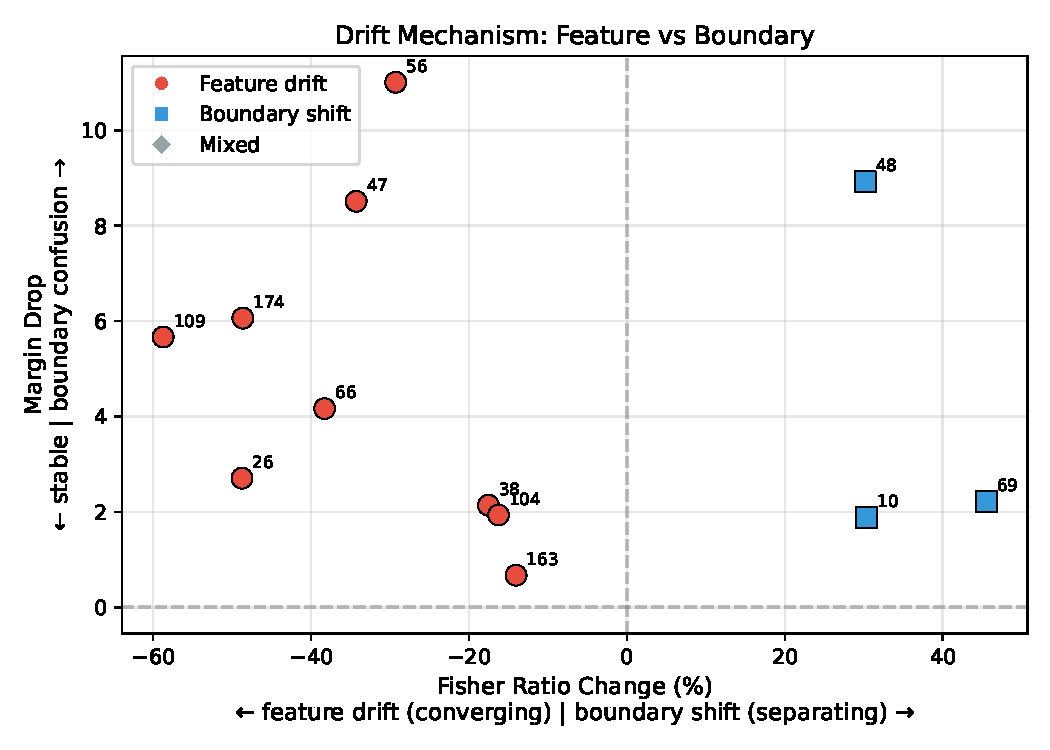
\includegraphics[width=\columnwidth]{drift_scatter.pdf}
\caption{Drift mechanism scatter plot for all 12 collapse classes. The x-axis shows the relative Fisher ratio change ($\Delta J$) from M4 to M12; the y-axis shows the margin drop (M4 margin $-$ M12 margin). Feature-drift classes (orange, $\Delta J < -10\%$) cluster in the left half; boundary-shift classes (blue, $\Delta J > +20\%$) appear on the right. All classes suffer large margin drops ($>$1.5), confirming that collapse is accompanied by decision-boundary erosion regardless of mechanism.}
\label{fig:drift_scatter}
\end{figure}

Figure~\ref{fig:drift_scatter} provides a complementary view: each collapse class is positioned by its Fisher ratio change (x-axis) and margin drop (y-axis), colored by mechanism type.
The clear spatial separation between feature-drift and boundary-shift classes validates the $\Delta J$-based classification rule and shows that margin drop alone cannot distinguish the two mechanisms.

\subsection{Why General TTA Methods Fail}
\label{sec:tta_eval}

We evaluate five TTA methods from computer vision on the same setup: Tent~\cite{wang2021tent}, EATA~\cite{niu2022eata}, SAR~\cite{niu2023sar}, CoTTA~\cite{wang2022cotta}, and NOTE~\cite{gong2022note}.
These are traffic-adapted implementations for 1D packet-sequence inputs, with necessary simplifications: EATA uses uniform Fisher importance (rather than per-sample Fisher computed from a held-out set), CoTTA uses Gaussian noise augmentation (as no standard augmentation pipeline exists for packet sequences), and NOTE uses a simplified prediction-balanced buffer without Instance-Aware BatchNorm.
Table~\ref{tab:tta} reports M12 results.

\begin{table}[t]
\centering
\caption{TTA baselines on CESNET-TLS-Year22 at M-2022-12 (traffic-adapted implementations, no labels). None of the tested variants repair collapse classes under our implementations.}
\label{tab:tta}
\small
\begin{tabular}{@{}l ccc@{}}
\toprule
Method & Macro-F1 & Collapse F1 & Stable F1 \\
\midrule
Static      & .629 & .028 & .903 \\
Tent        & .631 & .026 & .903 \\
EATA        & .629 & .028 & .903 \\
SAR         & .629 & .026 & .901 \\
CoTTA       & .629 & .027 & .903 \\
NOTE        & .630 & .027 & .902 \\
\bottomrule
\end{tabular}
\end{table}

These simplifications may underestimate the methods' potential; however, the near-zero collapse F1 across all tested variants---including Tent and SAR, which require no simplification---suggests a structural mismatch between confidence-based unsupervised adaptation and confident absorber--victim errors, rather than a simple hyperparameter artifact.
When an absorber class confidently captures a victim's predictions, entropy is \textit{low} (the model is confidently wrong), so entropy-based adaptation sees no signal to correct.
This negative result motivates the shift from unsupervised adaptation to label-efficient targeted repair.

To rule out suboptimal hyperparameters as an explanation, we sweep five learning rates from $10^{-5}$ to $10^{-3}$ (5 configurations per method).
The best collapse F1 across all configurations remains below 0.031 for every method (NOTE: 0.030, EATA: 0.028, CoTTA: 0.027, SAR: 0.027, Tent: 0.026), confirming that TTA failure is robust to learning-rate choice.
Higher learning rates cause Tent to catastrophically degrade (macro-F1 drops from 0.63 to 0.21 at $\text{lr}{=}10^{-3}$).

% ============================================================
\section{Method: Collapse-Aware Active Repair}
\label{sec:method}

\ours{} is a label-efficient repair framework comprising three stages: (1)~unsupervised monitoring of per-class health, (2)~active sample selection, and (3)~head fine-tuning with all-class replay and knowledge distillation.
Algorithm~\ref{alg:care} summarizes the procedure.

\subsection{Unsupervised Collapse Detection and Monitoring}
\label{sec:unsup_detect}

We propose a multi-signal collapse risk score computed entirely from model predictions on unlabeled data.
For each class $c$, we compare predictions between a reference period and the target period across five signals, all computed on samples \textit{predicted} as class $c$ (no true labels required):
\begin{enumerate}
  \item \textbf{Prediction count ratio}: $r_c = (n_c^{\text{tgt}}/N^{\text{tgt}}) / (n_c^{\text{ref}}/N^{\text{ref}})$. Collapsed classes lose predictions ($r_c \ll 1$).
  \item \textbf{Fr\'{e}chet Distance (FD)}: Feature distribution shift between periods for the predicted class region.
  \item \textbf{Margin drop}: Decrease in mean prediction margin (top-2 logit gap).
  \item \textbf{Confidence drop}: Decrease in mean prediction confidence.
  \item \textbf{Entropy rise}: Increase in mean prediction entropy.
\end{enumerate}

The collapse risk score combines these signals:
\begin{equation}
  s_c = w_1 \cdot \max(0, 1{-}r_c) + w_2 \cdot \tilde{d}_c + w_3 \cdot \tilde{m}_c + w_4 \cdot \tilde{f}_c + w_5 \cdot \tilde{e}_c
\end{equation}
where $\tilde{d}_c$, $\tilde{m}_c$, $\tilde{f}_c$, $\tilde{e}_c$ denote the MAD-normalized FD, margin drop, confidence drop, and entropy rise for class $c$, and $w = (0.40, 0.20, 0.15, 0.15, 0.10)$.
Weights were set as a fixed heuristic based on signal informativeness (count drop is the strongest single indicator), without access to target-period labels; labels are used only retrospectively to report detection precision and recall.
A sensitivity analysis (\S\ref{sec:discussion}) comparing manual, equal, and historically calibrated weights shows that detection F1 is robust to weight choice (0.563--0.625 on M12).

This module serves two deployment-critical roles:
\begin{itemize}
  \item \textbf{Monitoring}: It identifies \textit{which} classes are degrading, enabling targeted investigation by network operators.
  \item \textbf{Alerting}: Per-class risk scores inform \textit{when} repair should be considered, without requiring labeled data to detect drift.
\end{itemize}
Importantly, the detection module does \textit{not} guide replay class selection---all-class replay is the default (\S\ref{sec:replay_ablation}).

\subsection{Active Sample Selection}
\label{sec:sample_select}

From the target period, we select a budget $B$ of samples for labeling.
\textit{Margin sampling}---selecting samples with the smallest gap between the top-two logits---naturally concentrates on absorber--victim decision boundaries where labels are most informative.
\textit{BADGE}~\cite{ash2020badge} selects diverse uncertain samples via gradient embeddings and achieves higher performance at the cost of longer selection time (${\sim}$20 minutes vs.\ $<$1 second for margin on 330K samples).
We recommend BADGE as the strongest selector when compute permits, and margin as a lightweight alternative.

\subsection{Head Fine-Tuning with All-Class Source Replay}
\label{sec:ft_replay}

We fine-tune only the classification head $h_\theta$ using the selected target labels combined with $k{=}5$ samples per class from labeled reference-period data (all-class source replay, 890 samples total):
\begin{equation}
  \mathcal{L}_{\text{ft}} = \frac{1}{|D_{\text{target}} \cup D_{\text{replay}}|} \sum_{(x,y)} \ell_{\text{CE}}(h_\theta(f(x)), y)
\end{equation}
where $f(\cdot)$ is the frozen encoder.
All-class replay prevents the head from overfitting to the small target sample and maintains decision boundaries for all 178 classes. This is a critical advantage over targeted replay, as confirmed by the replay strategy ablation (\S\ref{sec:replay_ablation}).

\subsection{Knowledge Distillation}
\label{sec:distill}

On replay samples, we add a KL-divergence loss~\cite{hinton2015distilling} between the updated head $h_\theta$ and the original (frozen) head $h_{\theta_0}$:
\begin{equation}
  \mathcal{L}_{\text{KD}} = \frac{1}{|D_{\text{rpl}}|} \!\sum_{x \in D_{\text{rpl}}} D_{\text{KL}}\!\!\left(\sigma\!\!\left(\frac{h_{\theta_0}\!(f(x))}{T}\right) \!\Big\|\! \sigma\!\!\left(\frac{h_\theta\!(f(x))}{T}\right)\!\right)
\end{equation}
where $T$ is the temperature and $\sigma$ is softmax.
Distillation is applied only on replay samples (not target samples) because the teacher model's predictions on replay data represent its \textit{correct} behavior on the source distribution.
On target samples, the teacher's predictions may already reflect absorber-collapse errors, making them unsuitable as distillation targets.

\subsection{Combined Objective and Algorithm}

The full training loss is:
\begin{equation}
  \mathcal{L} = \mathcal{L}_{\text{ft}} + \lambda_{\text{KD}} \cdot \mathcal{L}_{\text{KD}}
\end{equation}

\begin{algorithm}[t]
\caption{\ours{}: Collapse-Aware Active Repair}
\label{alg:care}
\begin{algorithmic}[1]
\REQUIRE Source model $f, h_{\theta_0}$; reference predictions; target data $D_{\text{tgt}}$ (unlabeled); budget $B$
\STATE \textbf{Monitor:} Compute per-class risk scores $s_c$ (\S\ref{sec:unsup_detect}) from unlabeled predictions
\STATE \textbf{Alert:} If risk scores indicate drift, flag for operator review
\STATE Compute features and logits for $D_{\text{tgt}}$
\STATE Select $B$ samples via margin or BADGE; query labels $\to D_{\text{target}}$
\STATE Sample $D_{\text{replay}}$: $k{=}5$ per class from \textit{all} 178 training classes (890 total)
\STATE Initialize $h_\theta \leftarrow h_{\theta_0}$
\FOR{epoch $= 1, \ldots, E$}
  \STATE Sample minibatch from $D_{\text{target}} \cup D_{\text{replay}}$
  \STATE $\mathcal{L} \leftarrow \mathcal{L}_{\text{ft}} + \lambda_{\text{KD}} \cdot \mathcal{L}_{\text{KD}}$
  \STATE Update $\theta$ via gradient descent on $\mathcal{L}$
\ENDFOR
\RETURN Updated classifier $h_\theta$
\end{algorithmic}
\end{algorithm}


% ============================================================
\section{Experiments}
\label{sec:experiments}

\subsection{Experimental Setup}
\label{sec:exp_setup}

\textbf{Datasets.}
We use CESNET-TLS-Year22~\cite{hynek2024cesnet} (178 classes, 12 months, TLS traffic).
The dataset provides monthly partitions without per-flow timestamps, so all temporal analyses use month-level granularity.
We train on M-2022-3 and evaluate at M7, M9, M11, and M12.

\textbf{Baselines.}
We compare four categories:
(1)~\textit{Unsupervised TTA} (0 labels): Tent~\cite{wang2021tent}, EATA~\cite{niu2022eata}, SAR~\cite{niu2023sar}, CoTTA~\cite{wang2022cotta}, NOTE~\cite{gong2022note}.
(2)~\textit{Standard active learning} (1{,}000 labels + \ours{} components): entropy, coreset~\cite{sener2018coreset}, random.
(3)~\textit{Continual learning / drift adaptation} (1{,}000 labels): MEMENTO~\cite{cerasuolo2024memento}, ILETC~\cite{zhu2023iletc}, CADE~\cite{yang2021cade}, expanded head (\S\ref{sec:cl_baselines}).
(4)~\textit{\ours{} configurations} (1{,}000 labels): margin and BADGE~\cite{ash2020badge} with all-class replay.

\textbf{Evaluation protocol.}
All \ours{} results use \textit{strict evaluation}: the labeled samples selected for fine-tuning are \textit{excluded} from the test set before computing metrics.
Main results, ablation, and strategy comparisons are averaged over 5 random seeds; multi-period, prototype, and architecture studies use 3 seeds as noted.

\textbf{Metrics.}
(1)~Overall macro-F1 (all 178 classes);
(2)~collapse-class macro-F1 (12 classes with recall ${<}0.1$ in the static model at M12);
(3)~stable-class macro-F1 (20 classes with consistently high recall);
(4)~number of collapsed classes (recall ${<}0.1$);
(5)~per-class \textit{recovery status}: recovered ($R{\geq}0.30$), partial ($0.05{\leq}R{<}0.30$), or failed ($R{<}0.05$), where $R$ is the best recall across selection strategies.

\textbf{\ours{} configuration.}
Budget $B{=}1{,}000$, all-class replay with $k{=}5$ per class (890 samples), target repeat factor 2, $\lambda_{\text{KD}}{=}0.5$, $T{=}2.0$, head fine-tuning lr $10^{-3}$, 30 epochs.

\subsection{Main Results}
\label{sec:main_results}

Table~\ref{tab:main_results} presents the main comparison at M-2022-12 (nine months after training).

\begin{table}[t]
\centering
\caption{Main results on CESNET-TLS-Year22 at M-2022-12. TTA methods use no labels. Active methods use $B{=}1{,}000$ labels with all-class replay ($k{=}5$, 890 samples) and KD ($\lambda{=}0.5$). Strict eval, 5 seeds.}
\label{tab:main_results}
\scriptsize
\setlength{\tabcolsep}{3pt}
\begin{tabular}{@{}l cccc@{}}
\toprule
Method & Macro & Col.\ F1 & Stb.\ F1 & \#Col \\
\midrule
\multicolumn{5}{l}{\textit{No labeled target data:}} \\
Static          & .629 & .028 & .903 & 12 \\
Tent            & .631 & .026 & .903 & 12 \\
EATA            & .629 & .028 & .903 & 12 \\
SAR             & .629 & .026 & .901 & 11 \\
CoTTA           & .629 & .027 & .903 & 12 \\
NOTE            & .630 & .027 & .902 & 12 \\
\midrule
\multicolumn{5}{l}{\textit{Active ($B$=1000, all-class replay+KD, 5 seeds):}} \\
Entropy         & .628$\pm$.004 & .078$\pm$.015 & .887$\pm$.004 & 10.2 \\
Coreset         & .634$\pm$.005 & .116$\pm$.042 & .886$\pm$.007 & 8.8 \\
Random          & .668$\pm$.004 & .188$\pm$.024 & .892$\pm$.006 & 8.2 \\
\ours{}-Margin  & .686$\pm$.001 & .256$\pm$.009 & .892$\pm$.003 & 5.8 \\
\textbf{\ours{}-BADGE} & \textbf{.700$\pm$.003} & \textbf{.333$\pm$.040} & \textbf{.894$\pm$.004} & \textbf{4.0} \\
\bottomrule
\end{tabular}
\end{table}

Key findings:
\begin{itemize}
  \item None of the tested TTA methods address class collapse (collapse F1 $\leq$0.030), confirming that unsupervised adaptation cannot break confident absorber--victim confusion under our traffic-adapted implementations.
  \item Entropy and coreset selection are counterproductive: even with the same all-class replay + KD pipeline, entropy (0.628) and coreset (0.634) barely match the static baseline (0.629) because they select globally uncertain samples dominated by high-traffic classes, systematically avoiding the collapse boundary.
  \item \ours{}-BADGE achieves the best results: macro-F1 of $0.700{\pm}0.003$ ($+$11.3\%) and collapse F1 of $0.333{\pm}0.040$ ($12{\times}$ improvement). Significance: BADGE$>$margin ($p{=}0.001$), margin$>$random ($p{<}0.001$).
  \item \ours{}-Margin is a lightweight alternative ($<$1s selection) with lower variance ($\sigma_{\text{macro}}{=}0.001$ vs.\ 0.003) and strong performance (macro-F1: $0.686{\pm}0.001$).
\end{itemize}

\subsection{Component Ablation}
\label{sec:ablation}

Table~\ref{tab:ablation} presents a clean ablation of \ours{}'s three components.
All rows use margin selection with $B{=}1{,}000$, strict evaluation, and 5 seeds; only the repair components are varied.

\begin{table}[t]
\centering
\caption{Component ablation at M-2022-12 (margin, $B{=}1{,}000$, strict eval, 5 seeds). ``CE Rpl'' = all-class CE replay ($k{=}5$, 890 samples). KD is defined over $D_{\text{rpl}}$ (\S\ref{sec:distill}), so KD-marked rows always include replay; FT+KD uses targeted stable+absorber replay (150 samples). Replay-only and Rpl+KD use $B{=}0$.}
\label{tab:ablation}
\scriptsize
\setlength{\tabcolsep}{3pt}
\begin{tabular}{@{}l ccc ccc c@{}}
\toprule
 & \multicolumn{3}{c}{Components} & & & & \\
\cmidrule(lr){2-4}
Config. & Lbl & CE Rpl & KD & Macro & Col.\ F1 & Stb.\ F1 & \#Col \\
\midrule
Static & & & & .629 & .028 & \textbf{.903} & 12 \\
\midrule
Replay only & & \checkmark & & .563$\pm$.007 & .044$\pm$.019 & .816$\pm$.026 & 10.2 \\
Rpl+KD & & \checkmark & \checkmark & .618$\pm$.005 & .039$\pm$.016 & .888$\pm$.009 & 10.8 \\
\midrule
FT only & \checkmark & & & .638$\pm$.000 & .134$\pm$.001 & .839$\pm$.001 & 7.0 \\
FT+KD & \checkmark & & \checkmark & .670$\pm$.000 & .152$\pm$.007 & .887$\pm$.004 & 7.8 \\
FT+Rpl & \checkmark & \checkmark & & .659$\pm$.003 & .236$\pm$.010 & .854$\pm$.016 & 4.8 \\
\textbf{Full \ours{}} & \checkmark & \checkmark & \checkmark & \textbf{.686$\pm$.001} & \textbf{.256$\pm$.009} & .892$\pm$.003 & 5.8 \\
\bottomrule
\end{tabular}
\end{table}

\begin{figure}[t]
\centering
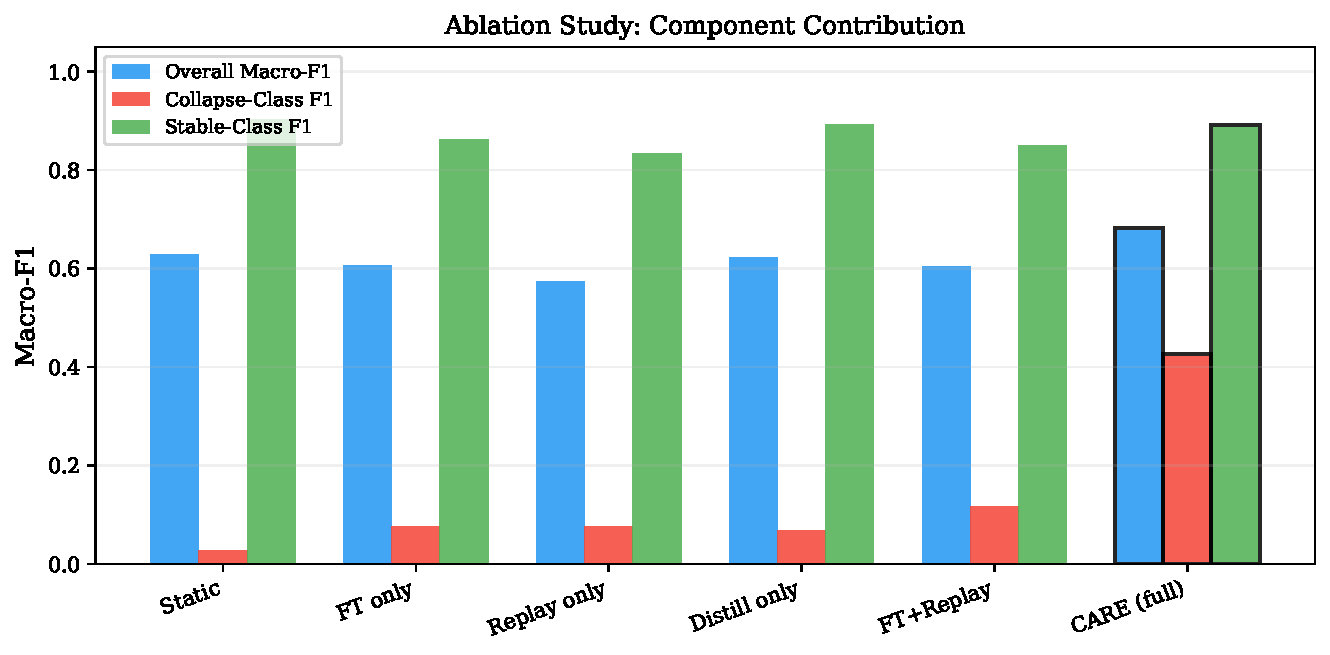
\includegraphics[width=\columnwidth]{fig_ablation_bar.pdf}
\caption{Component ablation visualization. Full \ours{} (rightmost) achieves the best trade-off between collapse repair (red) and stable-class preservation (green).}
\label{fig:ablation_bar}
\end{figure}

The table separates into three blocks.
\textbf{Without target labels} (Replay only, Rpl+KD): neither component alone can repair collapse---collapse F1 stays below .05---confirming that labeled target data is essential.
Rpl+KD preserves stable F1 (.888) nearly as well as the static model, while replay only degrades it (.816), showing that adding distillation to replay substantially reduces the noise that replay CE alone introduces.

\textbf{With target labels}, each component's contribution is isolated:
\begin{itemize}
  \item \textbf{FT only} (labels alone): Repairs collapse classes (.028$\to$.134) but severely damages stable classes (.903$\to$.839)---catastrophic forgetting from overfitting to 1{,}000 target samples.
  \item \textbf{FT+KD} (add distillation, with targeted replay as KD substrate): KD provides strong stable-class preservation (.839$\to$.887) with modest collapse improvement (.134$\to$.152), confirming its role as a regularizer.
  \item \textbf{FT+Rpl} (add replay): Replay substantially boosts collapse repair (.134$\to$.236) and macro-F1 (.638$\to$.659) by anchoring decision boundaries across all 178 classes, though stable-class recovery is partial (.839$\to$.854).
  \item \textbf{Full \ours{}} (all three): Combining labels, replay, and KD yields the best trade-off: macro-F1 reaches .686, collapse F1 .256, and stable F1 recovers to .892---close to the static baseline (.903).
\end{itemize}
Each component serves a distinct role: target labels provide the repair signal, all-class replay prevents forgetting across 178 classes, and KD regularizes the head to preserve stable-class behavior.

\subsection{Selection Strategy Comparison}
\label{sec:al_baselines}

\begin{figure}[t]
\centering
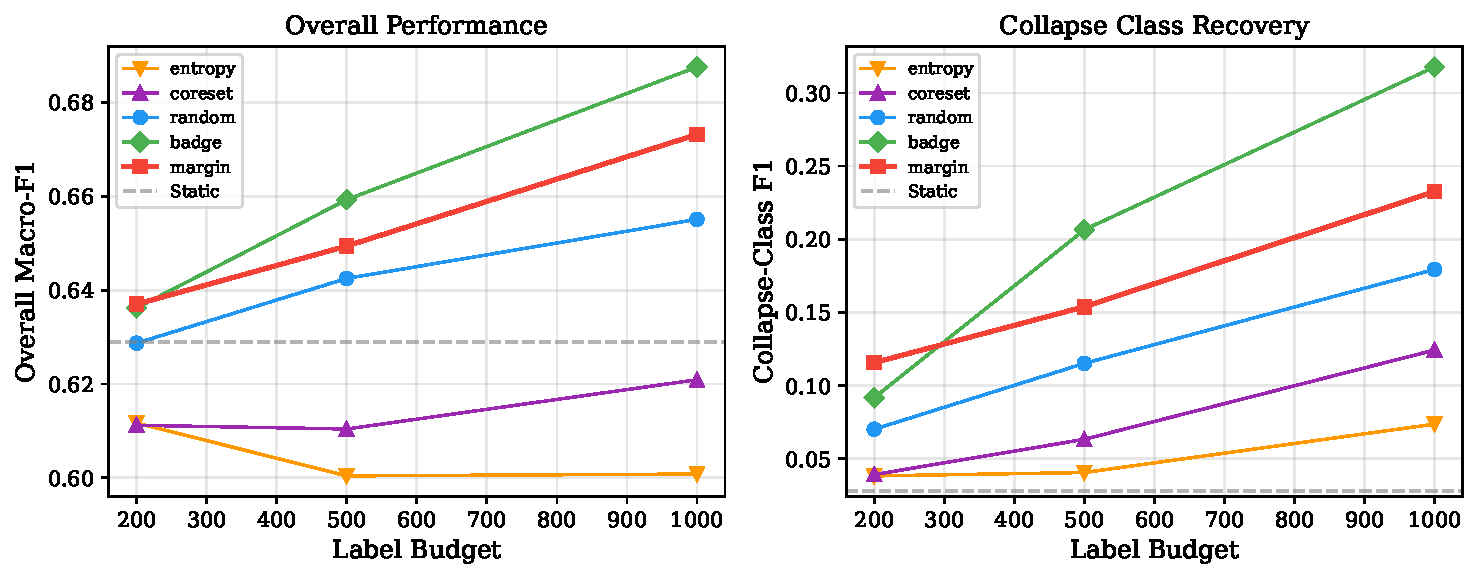
\includegraphics[width=\columnwidth]{fig_strategy_comparison.pdf}
\caption{Selection strategy comparison. Margin and BADGE consistently outperform entropy and coreset, which fall below the static baseline.}
\label{fig:strategy_comparison}
\end{figure}

Margin sampling targets samples where the top-two predictions are close, naturally concentrating on absorber--victim boundaries.
BADGE~\cite{ash2020badge} achieves the highest collapse F1 ($0.333{\pm}0.040$)---30\% above margin ($0.256{\pm}0.009$)---and macro-F1 ($0.700{\pm}0.003$ vs.\ $0.686{\pm}0.001$).
We recommend BADGE for scheduled maintenance and margin for resource-constrained deployments.

Table~\ref{tab:per_class_recovery} shows per-class recovery: 6 classes are fully recovered ($R{\geq}0.30$), 5 partial, and class~109 remains unrecovered (late onset, low support $n{=}393$).
Both selectors allocate very few labels to collapse classes (0--13 out of 1{,}000); repair succeeds primarily through all-class replay anchoring rather than direct label allocation.

\begin{table*}[t]
\centering
\caption{Per-class recovery at M-2022-12 ($B{=}1{,}000$, all-class replay $k{=}5$, strict eval, 5 seeds). Status is assigned by the best recall across Margin and BADGE: recovered ($R{\geq}0.30$), partial ($0.05{\leq}R{<}0.30$), failed ($R{<}0.05$). Selected = mean target labels allocated to that class.}
\label{tab:per_class_recovery}
\scriptsize
\setlength{\tabcolsep}{3.5pt}
\begin{tabular}{@{}r r r cc cc cc rr l@{}}
\toprule
& & & \multicolumn{2}{c}{Static} & \multicolumn{2}{c}{\ours{}-Margin} & \multicolumn{2}{c}{\ours{}-BADGE} & \multicolumn{2}{c}{Selected} & \\
\cmidrule(lr){4-5} \cmidrule(lr){6-7} \cmidrule(lr){8-9} \cmidrule(lr){10-11}
Class & Abs. & $n$ & Recall & F1 & Recall & F1 & Recall & F1 & Marg & BADGE & Status \\
\midrule
56  & 96  & 12137 & .000 & .001 & .722$\pm$.030 & .784$\pm$.007 & \textbf{.793$\pm$.015} & \textbf{.829$\pm$.019} & 12.0 & 13.6 & recovered \\
163 & 46  &  1741 & .016 & .026 & .143$\pm$.028 & .168$\pm$.021 & \textbf{.226$\pm$.125} & \textbf{.235$\pm$.110} &  3.0 &  4.8 & partial \\
174 &  2  &  1507 & .000 & .000 & \textbf{.195$\pm$.005} & \textbf{.262$\pm$.011} & .029$\pm$.036 & .044$\pm$.054 &  4.0 &  1.6 & partial \\
48  & 14  &  3361 & .001 & .002 & .437$\pm$.008 & .568$\pm$.006 & \textbf{.722$\pm$.209} & \textbf{.767$\pm$.130} &  4.0 &  4.8 & recovered \\
38  & 45  &   193 & .052 & .090 & \textbf{.656$\pm$.085} & \textbf{.410$\pm$.051} & .242$\pm$.248 & .210$\pm$.188 &  3.0 &  1.2 & recovered \\
69  & 105 &  1866 & .005 & .008 & .031$\pm$.016 & .042$\pm$.019 & \textbf{.157$\pm$.182} & \textbf{.177$\pm$.196} &  3.0 &  2.4 & partial \\
104 &  2  &  1744 & .010 & .016 & \textbf{.703$\pm$.039} & \textbf{.664$\pm$.028} & .604$\pm$.138 & .594$\pm$.065 &  8.0 &  3.6 & recovered \\
47  &  5  &   618 & .000 & .000 & .002$\pm$.002 & .004$\pm$.003 & \textbf{.404$\pm$.180} & \textbf{.462$\pm$.150} &  0.0 &  2.2 & recovered \\
66  & 71  &  1955 & .001 & .002 & .001$\pm$.000 & .002$\pm$.001 & \textbf{.133$\pm$.105} & \textbf{.144$\pm$.108} &  1.0 &  4.2 & partial \\
10  & 156 &  1004 & .098 & .162 & .074$\pm$.027 & .121$\pm$.039 & \textbf{.389$\pm$.193} & \textbf{.441$\pm$.172} &  0.0 &  1.8 & recovered \\
109 & 71  &   393 & .000 & .000 & .000$\pm$.000 & .000$\pm$.000 & .000$\pm$.000 & .000$\pm$.000 &  0.0 &  1.6 & failed \\
26  & 13  &   807 & .022 & .025 & .035$\pm$.010 & .046$\pm$.010 & \textbf{.125$\pm$.125} & \textbf{.087$\pm$.062} &  1.0 &  2.6 & partial \\
\midrule
\multicolumn{3}{@{}l}{Macro (12 classes)} & .017 & .028 & .250 & .256 & \textbf{.319} & \textbf{.332} & & & 6R/5P/1F \\
\bottomrule
\end{tabular}
\end{table*}

\begin{figure*}[t]
\centering
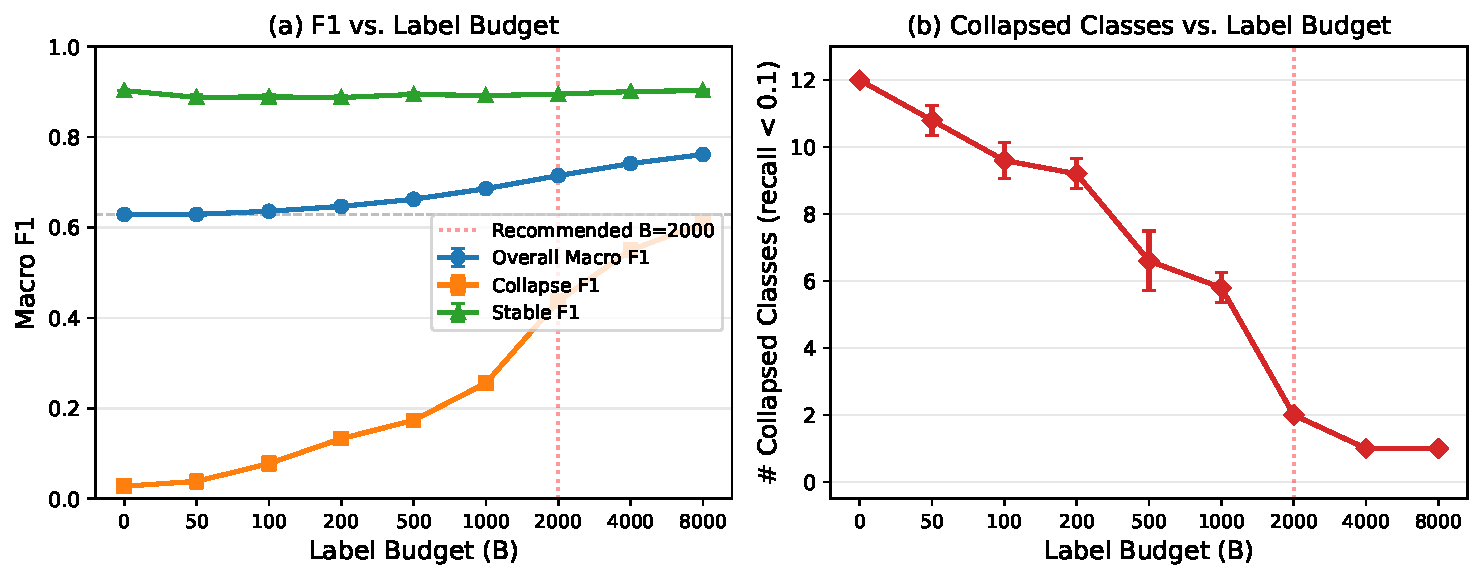
\includegraphics[width=\textwidth]{budget_curve.pdf}
\caption{Label budget vs.\ performance (margin, 5 seeds, error bars). Left: Overall, collapse, and stable macro F1. Right: number of collapsed classes (recall $< 0.1$). The knee at $B{=}2{,}000$ reduces collapsed classes from 12 to 2; beyond $B{=}4{,}000$ gains are marginal.}
\label{fig:budget_sweep}
\end{figure*}

Figure~\ref{fig:budget_sweep} shows performance as a function of label budget $B \in \{0, 50, 100, 200, 500, 1000, 2000, 4000, 8000\}$.
Collapse F1 improves steadily from 0.028 (static) to $0.609{\pm}0.007$ at $B{=}8{,}000$, while stable-class F1 remains above 0.89 throughout, confirming that repair does not harm non-collapsed classes.
We recommend $B{=}2{,}000$ as the operating point: it raises collapse F1 to $0.437{\pm}0.004$ (a $16{\times}$ improvement over static) and reduces collapsed classes from 12 to 2, at moderate labeling cost.
Beyond $B{=}4{,}000$ ($0.550{\pm}0.007$), gains are marginal ($+0.014$ per additional 1{,}000 labels vs.\ $+0.181$ in the 1{,}000$\to$2{,}000 range).
All comparative experiments (Tables~\ref{tab:main_results}--\ref{tab:cl_baselines}) use $B{=}1{,}000$ to maintain a uniform low-budget baseline across methods; the budget curve shows that practitioners with larger annotation budgets can achieve substantially better collapse repair.

\subsection{Replay Strategy Ablation}
\label{sec:replay_ablation}

A key design choice is whether to replay all classes or only detected/targeted classes.
Table~\ref{tab:replay_ablation} compares replay strategies under matched conditions (margin, $B{=}1{,}000$, 5 seeds).

\begin{table}[t]
\centering
\caption{Replay strategy ablation (margin, $B$=1000, 5 seeds). ``Targeted'' replays only stable and absorber classes (oracle list); all-class $k{=}5$ is best, showing advantage is class-coverage breadth, not volume.}
\label{tab:replay_ablation}
\scriptsize
\setlength{\tabcolsep}{3pt}
\begin{tabular}{@{}l cc c@{}}
\toprule
Replay Config. & Macro & Col.\ F1 & $n_{\text{rpl}}$ \\
\midrule
All-class $k{=}5$ (890) & \textbf{.686$\pm$.001} & \textbf{.256$\pm$.009} & 890 \\
Targeted $k{=}30$ (${\sim}$900) & .678$\pm$.001 & .243$\pm$.003 & $\sim$900 \\
All-class $k{=}1$ (178) & .680$\pm$.003 & .231$\pm$.015 & 178 \\
\bottomrule
\end{tabular}
\end{table}

All-class replay with $k{=}5$ yields the best results (.686 macro-F1).
To rule out the confound that all-class replay simply uses more samples, we match the total replay budget: targeted replay with $k{=}30$ (${\approx}$900 samples, matched budget) achieves only .678, while all-class $k{=}1$ (178 samples) achieves .680.
This confirms that the advantage comes from \textit{class-coverage breadth}, not replay volume: anchoring all 178 class boundaries is more effective than concentrating replay on a subset.

This finding also clarifies the role of the detection module.
Its value is \textit{not} in guiding replay class selection---all-class replay is strictly better---but in two deployment roles: (1)~identifying \textit{which} classes are degrading for targeted investigation, and (2)~flagging \textit{when} repair should be considered by the operator.

\subsection{Comparison with Continual Learning Baselines}
\label{sec:cl_baselines}

To situate \ours{} against continual-learning and drift-adaptation methods, we adapt four representative approaches to our collapse-repair setting (Table~\ref{tab:cl_baselines}).
All methods use the same evaluation protocol (margin selection, $B{=}1{,}000$, strict eval, 5 seeds). Except for MEMENTO (which fine-tunes the full model), all methods share the same frozen encoder and differ in how the classification head is updated or what replay data is used.

\begin{itemize}
  \item \textbf{MEMENTO}~\cite{cerasuolo2024memento}: Full-model fine-tuning (encoder + head) with KD on all-class replay. MEMENTO's output rectification reduces to a no-op when replaying all classes, so we report the core mechanism only.
  \item \textbf{ILETC}~\cite{zhu2023iletc}: A conditional WGAN-GP generates synthetic replay features per class; the head is fine-tuned on target labels + GAN-generated replay without KD.
  \item \textbf{CADE-score}~\cite{yang2021cade}: A contrastive autoencoder computes per-sample drift scores; the top-$B$ highest-scoring samples are selected for labeling instead of margin sampling. Repair uses the same head fine-tuning + replay + KD pipeline as \ours{}.
  \item \textbf{Expanded head}: The single-layer head (Linear(256, $C$)) is replaced by a two-layer head (Linear(256, 512)$\to$ReLU$\to$Linear(512, $C$)), initialized via a dual-channel decomposition that exactly reproduces the original head's output before fine-tuning.
\end{itemize}

\begin{table}[t]
\centering
\caption{Continual learning and drift-adaptation baselines at M-2022-12 (margin, $B{=}1{,}000$, strict eval, 5 seeds). \ours{}-Margin and \ours{}-BADGE are reproduced from Table~\ref{tab:main_results} for comparison.}
\label{tab:cl_baselines}
\scriptsize
\setlength{\tabcolsep}{3pt}
\begin{tabular}{@{}l cccc@{}}
\toprule
Method & Macro & Col.\ F1 & Stb.\ F1 & \#Col \\
\midrule
Static & .629 & .028 & \textbf{.903} & 12.0 \\
\midrule
\multicolumn{5}{l}{\textit{CL / drift baselines (margin, same budget):}} \\
CADE-score~\cite{yang2021cade}     & .637$\pm$.004 & .118$\pm$.015 & .889$\pm$.003 & 9.0 \\
ILETC-GAN~\cite{zhu2023iletc}     & .650$\pm$.004 & .219$\pm$.010 & .851$\pm$.009 & 5.4 \\
ILETC-real                         & .659$\pm$.003 & .236$\pm$.010 & .854$\pm$.016 & 4.8 \\
Expanded head                      & .673$\pm$.003 & .307$\pm$.005 & .871$\pm$.008 & 4.8 \\
MEMENTO~\cite{cerasuolo2024memento}& .678$\pm$.003 & .255$\pm$.004 & .892$\pm$.003 & 6.0 \\
\midrule
\ours{}-Margin & .686$\pm$.001 & .256$\pm$.009 & .892$\pm$.003 & 5.8 \\
\textbf{\ours{}-BADGE} & \textbf{.700$\pm$.003} & \textbf{.333$\pm$.040} & .894$\pm$.004 & \textbf{4.0} \\
\bottomrule
\end{tabular}
\end{table}

Three findings emerge:
\begin{itemize}
  \item \textbf{Full-model fine-tuning does not help.} MEMENTO achieves comparable collapse F1 to \ours{}-Margin (.255 vs.\ .256) but lower macro-F1 (.678 vs.\ .686), confirming that updating encoder parameters is underconstrained with only 1{,}000 labels. This validates \ours{}'s head-only design.
  \item \textbf{GAN-generated replay is inferior to real replay.} ILETC-GAN underperforms ILETC-real on both macro-F1 (.650 vs.\ .659) and collapse F1 (.219 vs.\ .236), and both trail \ours{}-Margin. The 256-dim feature space appears too complex for the conditional WGAN-GP to faithfully reproduce. Both ILETC variants also suffer notable stable-class degradation (.851--.854 vs.\ .892) because they omit knowledge distillation.
  \item \textbf{Capacity expansion helps collapse but hurts stability.} The expanded head achieves the highest collapse F1 among non-BADGE methods (.307), reducing collapsed classes from 12 to 4.8. However, this comes at the cost of stable-class F1 (.871 vs.\ .892) and overall macro-F1 (.673 vs.\ .686). The result suggests that head capacity is a contributing factor in collapse, but \ours{}-BADGE achieves better collapse repair (.333) \textit{without} sacrificing stable-class performance.
\end{itemize}

CADE-score selection performs worst (.118 collapse F1), consistent with the observation that drift scores identify \textit{anomalous} samples rather than \textit{informative} boundary samples. Overall, \ours{}-BADGE remains the best trade-off across all metrics.

\subsection{Multi-Period Analysis}
\label{sec:multi_period}

Table~\ref{tab:multiperiod} shows \ours{}'s effectiveness across four time points with increasing drift severity.

\begin{table}[t]
\centering
\caption{Multi-period results (margin, $B$=1000, all-class replay $k{=}5$, 3 seeds). Fixed 12-class eval set. Benefit increases with drift severity.}
\label{tab:multiperiod}
\scriptsize
\setlength{\tabcolsep}{3pt}
\begin{tabular}{@{}l cc cc c@{}}
\toprule
& \multicolumn{2}{c}{Static} & \multicolumn{2}{c}{\ours{}} & \\
\cmidrule(lr){2-3} \cmidrule(lr){4-5}
Period & Macro & Col. & Macro & Col. & $\Delta$ \\
\midrule
M7 (light)   & .740 & .503 & .776$\pm$.003 & .633$\pm$.028 & +.036 \\
M9 (medium)  & .691 & .280 & .739$\pm$.003 & .392$\pm$.005 & +.048 \\
M11 (heavy)  & .649 & .145 & .708$\pm$.002 & .408$\pm$.016 & +.060 \\
M12 (severe) & .629 & .028 & .686$\pm$.002 & .255$\pm$.012 & +.057 \\
\bottomrule
\end{tabular}
\end{table}

\ours{} is effective at all drift levels, with increasing benefit as drift severity grows (M7: +0.036; M11: +0.060).
Collapse repair is most successful at M7, where the absorber--victim separation in feature space is still partially intact (collapse F1 = 0.633 vs.\ 0.255 at M12).
This suggests that \textit{early intervention is more effective}: repairing at M7 yields better per-class recovery than waiting until M12.

\subsection{Detection Evaluation}
\label{sec:detection_eval}

\textbf{Signal ablation.}
Table~\ref{tab:detect_signals} shows how each signal contributes to detection accuracy at M12.
The detection ground truth uses the same collapse definition as repair evaluation: recall~${<}\,0.1$ with support~${\geq}\,50$, yielding 12 ground-truth collapsed classes.
The detector selects the 20 highest-risk classes ($k{=}20$).

\begin{table}[t]
\centering
\caption{Detection signal ablation on M4$\to$M12 (12 ground-truth classes, no labels used, $k{=}20$).}
\label{tab:detect_signals}
\small
\begin{tabular}{@{}l ccc@{}}
\toprule
Signal Combination & Precision & Recall & F1 \\
\midrule
FD only & .350 & .583 & .438 \\
Count + FD & .450 & .750 & .563 \\
Count + FD + margin + conf & .400 & .667 & .500 \\
All 5 signals & \textbf{.500} & \textbf{.833} & \textbf{.625} \\
\bottomrule
\end{tabular}
\end{table}

Count drop and FD provide the primary detection signal (F1 = 0.563); adding margin and confidence alone does not improve detection, but entropy rise contributes a complementary signal that lifts recall from 0.750 to 0.833 and F1 from 0.563 to 0.625.

\textbf{Detection across drift levels.}
Table~\ref{tab:trigger} evaluates detection consistency as a diagnostic monitor across four time points.

\begin{table}[t]
\centering
\caption{Detection across drift levels ($k{=}20$, recall${<}0.1$, support${\geq}50$). Recall is $\geq$0.80 at all time points; precision improves with drift severity.}
\label{tab:trigger}
\small
\begin{tabular}{@{}l cccc@{}}
\toprule
Period & GT & Precision & Recall & F1 \\
\midrule
M7 (light)   & 5  & .200 & .800 & .320 \\
M9 (medium)  & 8  & .350 & .875 & .500 \\
M11 (heavy)  & 10 & .450 & .900 & .600 \\
M12 (severe) & 12 & .500 & .833 & .625 \\
\bottomrule
\end{tabular}
\end{table}

Recall is $\geq$0.80 at all periods; precision increases with drift severity (0.20 at M7 to 0.50 at M12) as more classes genuinely collapse.
The two consistently missed classes are 38 (small support) and 163 (gradual drift).

\subsection{Robustness and Extensions}
\label{sec:robustness}

\textbf{Architecture independence.}
\label{sec:bn_verify}
\label{sec:transformer}
To confirm that TTA failure is not caused by our use of GroupNorm, we train an identical CNN with BatchNorm (BN): BN-Adapt~\cite{schneider2020bn} raises macro-F1 by only 0.009 while collapse F1 stays at 0.032, and NOTE catastrophically degrades (macro-F1: 0.042). \ours{}-Margin still improves the BN model substantially (.613$\to$.665 macro, .030$\to$.314 collapse).
We also train a Transformer backbone~\cite{vaswani2017attention} (4-layer, 4-head, 256-dim): \ours{} achieves $.767{\pm}.001$ macro-F1 and $.401{\pm}.003$ collapse F1, a larger gain than on the CNN (+0.097 vs.\ +0.057), likely because richer features provide better material for head-only repair.

\textbf{Prototype replay.}
\label{sec:proto_replay}
For privacy-sensitive deployments, we replace stored samples with class prototypes (mean feature vectors + Gaussian noise, 178~KB total).
Prototype replay achieves 98.7\% of real replay's macro-F1 ($0.664{\pm}0.002$ vs.\ $0.673{\pm}0.001$, 3 seeds), demonstrating exemplar-free operation with minimal loss.

\textbf{Statistical significance.}
\label{sec:significance}
Paired $t$-tests (5 seeds) confirm: margin $>$ random ($p{<}0.001$) and BADGE $>$ margin ($p{=}0.001$).
A retraining audit ($3{\times}3{=}9$ runs) yields training-seed variance $\sigma_{\text{macro}}{=}0.0006$, confirming that absorber-collapse is a data property, not a training artifact.


% ============================================================
\section{Discussion}
\label{sec:discussion}

\textbf{Label cost and deployment model.}
\ours{} requires 1{,}000 target labels per repair cycle ($<$0.3\% of the ${\sim}$330K monthly test set) plus 890 all-class replay samples from a labeled reference period.
In our experiments, we use M4 as the reference period; a comparison (5 seeds, margin, $B{=}1{,}000$) shows that using the training month M3 yields equivalent results across all metrics: macro-F1 $0.672{\pm}0.002$ vs.\ $0.673{\pm}0.001$, collapse F1 $0.234{\pm}0.002$ vs.\ $0.232{\pm}0.003$, stable F1 $0.887{\pm}0.003$ vs.\ $0.885{\pm}0.003$.
Replay can therefore reuse training data at zero additional labeling cost.
In ISP deployment, target labels can be obtained through DPI-based labeling on a monitored subnet, SNI-based ground truth for TLS traffic, or periodic manual verification.
In deployment, repair would be initiated when the detection module signals drift, so labeling cost is incurred only when needed.

\textbf{Detection false positives and deployment cost.}
The detection module achieves precision 0.50 at M12, meaning half of flagged classes are false positives.
However, false positives do \textit{not} cause unnecessary per-class labeling: the detection module signals a single repair cycle covering all classes, not per-class repairs.
Once repair is initiated, the 1{,}000-label active selection and all-class replay address all collapsed classes simultaneously regardless of which specific classes the detector flagged.
The detection module's primary deployment value is its high recall ($\geq$0.80 across all evaluated periods), reducing the risk of missed collapse events.

\textbf{Stable-class trade-off.}
Stable-class F1 decreases from 0.903 (Static) to 0.892 ($-$1.2\%) under Full \ours{} with all-class replay.
The ablation shows each component's role: without replay and distillation, degradation is severe (0.839); with the full method, stable F1 recovers to 0.892, limiting degradation to ${\leq}$1.2\%---an acceptable trade-off for $12{\times}$ collapse recovery.

\textbf{Deployability.}
\ours{} is designed for deployment with minimal operator intervention:
(1)~the detection module monitors class health without labels, flagging at-risk classes for operator review;
(2)~margin selection requires no absorber knowledge;
(3)~all-class replay from labeled reference-period data is the default (equivalently, training data; \S\ref{sec:discussion}), with prototype replay as a privacy-preserving alternative;
(4)~repair completes in ${\sim}$3 minutes on an NVIDIA RTX 3090.
The updated head is swapped in atomically after training completes offline, so repair does not interrupt online inference.

\textbf{Fine-tuning depth.}
We compare head-only repair (default) with full-model fine-tuning (encoder + head, lr scaled by $0.1{\times}$) under the same 1{,}000-label budget (margin, all-class replay $k{=}5$, 5 seeds).
Full fine-tuning achieves macro-F1 of $0.678{\pm}0.001$ and collapse F1 of $0.256{\pm}0.005$, while head-only repair reaches $0.686{\pm}0.001$ and $0.256{\pm}0.009$ respectively.
Collapse recovery is comparable, but full fine-tuning slightly hurts overall and stable-class performance under the same label budget, likely because the encoder's ${\sim}$200K parameters are underconstrained with only 1{,}000 labels.
This supports our design choice of freezing the encoder and repairing only the classification head.

\textbf{Limitations.}
Per-class analysis (Table~\ref{tab:per_class_recovery}) reveals that 6 of 12 collapse classes are fully recovered, 5 show partial recovery, and class~109 remains unrecovered across all seeds, suggesting that \ours{} is most effective when the victim retains some discriminative features at the encoder level.
Since \ours{} updates only the classification head, it cannot recover classes whose encoder-level features have fully merged with the absorber---for such extreme cases, encoder adaptation or retraining may be necessary at higher cost.
\ours{} addresses \textit{existing} class collapse but does not handle emerging new classes---a complementary problem addressed by class-incremental methods~\cite{cai2024cpn}.

\textbf{Computational cost.}
A full \ours{}-Margin repair cycle takes approximately 3 minutes: feature extraction (${\sim}$40s for 330K samples), margin selection ($<$1s), and head fine-tuning (30 epochs, ${\sim}$90s with 1{,}000 target + 890 replay samples).
BADGE selection adds ${\sim}$20 minutes for PCA-accelerated k-means++ over gradient embeddings.
Both are negligible compared to full model retraining (${\sim}$2 hours).

\textbf{Detection weight sensitivity.}
We compare three weight configurations for the unsupervised collapse detection module: \textit{manual} $[.40,.20,.15,.15,.10]$ (default), \textit{equal} $[.20,.20,.20,.20,.20]$, and \textit{calibrated} weights optimized via grid search on M7+M9 ground-truth labels (supervised historical calibration, tested on held-out M11/M12 only).
On M12, manual and calibrated both achieve detection F1 of 0.625 (precision 0.50, recall 0.83), while equal weights reach 0.563 (precision 0.45, recall 0.75).
The calibrated weights $[.30,.00,.00,.40,.30]$ drop Fisher-ratio and margin signals entirely, relying on count change, confidence, and entropy alone---yet match the manual default.
This confirms the detection module is robust to weight choice; the manual default is a good operating point without requiring labeled calibration data.

\textbf{Calibration baseline.}
Temperature scaling ($T^*{=}1.11$, learned on validation data) changes zero predictions out of 1.32M test samples, leaving all metrics identical.
This confirms that class collapse arises from confident misprediction---the model is wrong with high confidence---and cannot be addressed by post-hoc calibration.

\textbf{Collapse threshold sensitivity.}
We vary the collapse definition threshold $\tau \in \{0.05, 0.10, 0.15\}$ (recall below which a class is considered collapsed) and minimum support $s \in \{50, 100, 200\}$ (5 seeds each).
The number of identified collapse classes ranges from 10 ($\tau{=}0.05$) to 13 ($\tau{=}0.15$), but \ours{}'s improvement is stable: collapse-class F1 gains $\Delta{=}0.208$--$0.246$ across all configurations.
Varying support from 50 to 100 has no effect; $s{=}200$ drops one borderline class (38) at $\tau{=}0.10$.
This confirms that our collapse definition and repair effectiveness are not artifacts of a particular threshold choice.

\textbf{Week-10 data collection change.}
CESNET-TLS-Year22 has a known distribution shift at week~10 due to a flow exporter update~\cite{hynek2024cesnet}.
This affects all methods equally and does not invalidate comparative results.


% ============================================================
\section{Conclusion}
\label{sec:conclusion}

We identified the absorber-collapse pattern---a previously unstudied failure mode where dominant classes systematically absorb victim-class predictions under concept drift in encrypted traffic classifiers.
On CESNET-TLS-Year22, 12 of 178 classes collapse below 0.1 recall within nine months.
We showed that unsupervised TTA methods do not address this failure under our tested configurations (collapse F1 ${<}0.03$) and that entropy/coreset active learning strategies are counterproductive, establishing class collapse as a distinct problem requiring targeted intervention.

Our collapse-aware evaluation---per-class recovery status, collapse vs.\ stable F1, and strict query exclusion---reveals failure modes invisible to aggregate metrics.
We proposed \ours{}, a label-efficient maintenance protocol with three components: (1)~few-label head fine-tuning with margin or BADGE selection, (2)~all-class source replay, and (3)~knowledge distillation.
An unsupervised detection module monitors per-class health as a diagnostic monitor; experiments evaluate repair on known drift periods identified by this module.
Under strict evaluation (five seeds), \ours{}-BADGE raises macro-F1 from 0.629 to $0.700{\pm}0.003$ and collapse F1 from 0.028 to $0.333{\pm}0.040$ using only 1{,}000 target labels plus 890 replay samples; \ours{}-Margin achieves $0.686{\pm}0.001$ with sub-second selection.
A clean component ablation confirms that each ingredient contributes independently: FT alone reaches 0.638, adding all-class CE replay lifts it to 0.659, and adding KD achieves 0.686.
A replay strategy ablation shows that all-class replay outperforms targeted replay even at matched budgets (0.686 vs.\ 0.678 at ${\sim}$900 samples), establishing that class-coverage breadth matters more than targeted volume.
The framework is consistent across drift severity (M7--M12), architectures (CNN/Transformer), and training seeds.

% ============================================================
\bibliographystyle{IEEEtran}
\bibliography{references}

\end{document}
